% Created by tikzDevice version 0.12.3.1 on 2022-11-14 16:57:45
% !TEX encoding = UTF-8 Unicode
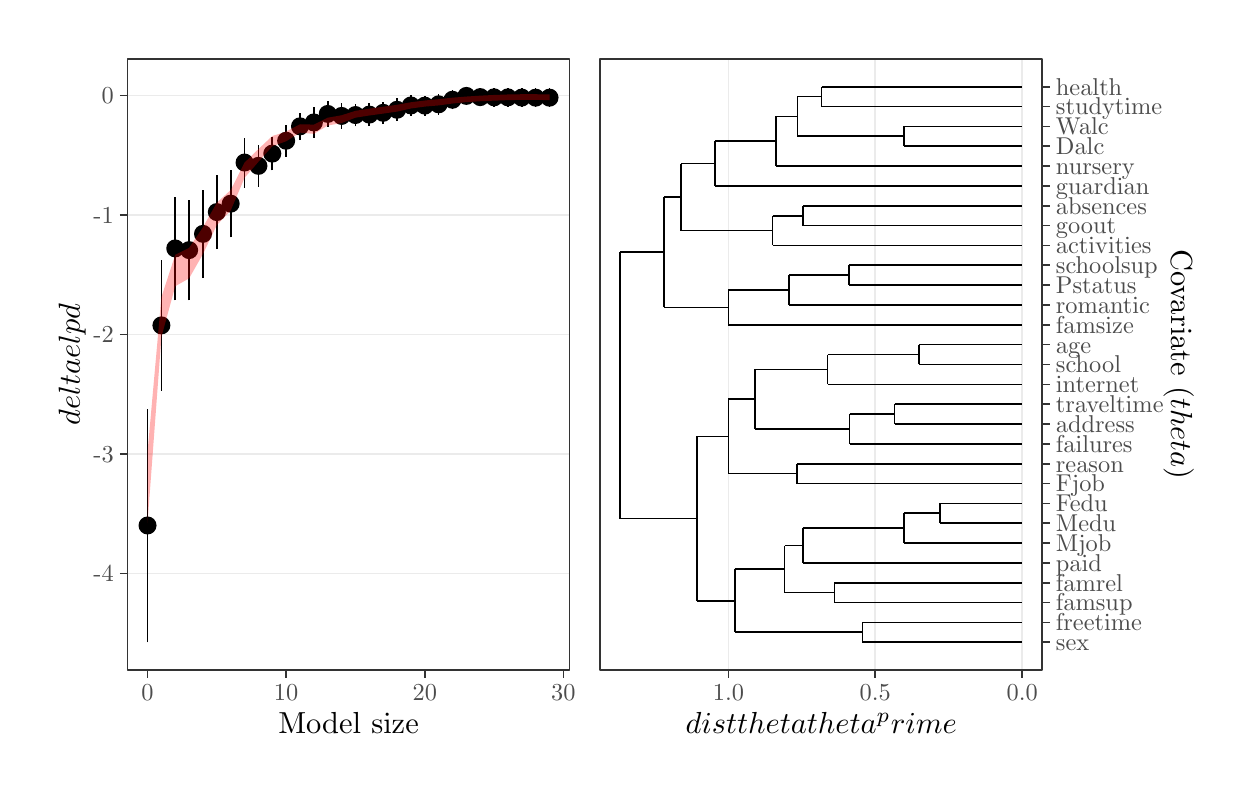
\begin{tikzpicture}[x=1pt,y=1pt]
\definecolor{fillColor}{RGB}{255,255,255}
\begin{scope}
\definecolor{drawColor}{RGB}{255,255,255}
\definecolor{fillColor}{RGB}{255,255,255}

\path[draw=drawColor,line width= 0.6pt,line join=round,line cap=round,fill=fillColor] (  0.00,  0.00) rectangle (433.62,268.00);
\end{scope}
\begin{scope}
\definecolor{drawColor}{RGB}{255,255,255}
\definecolor{fillColor}{RGB}{255,255,255}

\path[draw=drawColor,line width= 0.6pt,line join=round,line cap=round,fill=fillColor] (  5.50,  5.50) rectangle (201.03,262.50);
\end{scope}
\begin{scope}
\definecolor{fillColor}{RGB}{255,255,255}

\path[fill=fillColor] ( 35.75, 36.19) rectangle (195.53,257.00);
\definecolor{drawColor}{gray}{0.92}

\path[draw=drawColor,line width= 0.6pt,line join=round] ( 35.75, 71.10) --
	(195.53, 71.10);

\path[draw=drawColor,line width= 0.6pt,line join=round] ( 35.75,114.29) --
	(195.53,114.29);

\path[draw=drawColor,line width= 0.6pt,line join=round] ( 35.75,157.47) --
	(195.53,157.47);

\path[draw=drawColor,line width= 0.6pt,line join=round] ( 35.75,200.66) --
	(195.53,200.66);

\path[draw=drawColor,line width= 0.6pt,line join=round] ( 35.75,243.84) --
	(195.53,243.84);
\definecolor{drawColor}{RGB}{0,0,0}

\path[draw=drawColor,line width= 0.6pt,line join=round] ( 43.01, 46.22) -- ( 43.01,130.61);

\path[draw=drawColor,line width= 0.6pt,line join=round] ( 48.02,137.03) -- ( 48.02,184.40);

\path[draw=drawColor,line width= 0.6pt,line join=round] ( 53.03,169.79) -- ( 53.03,207.27);

\path[draw=drawColor,line width= 0.6pt,line join=round] ( 58.04,169.79) -- ( 58.04,206.04);

\path[draw=drawColor,line width= 0.6pt,line join=round] ( 63.05,177.84) -- ( 63.05,209.75);

\path[draw=drawColor,line width= 0.6pt,line join=round] ( 68.05,188.32) -- ( 68.05,215.01);

\path[draw=drawColor,line width= 0.6pt,line join=round] ( 73.06,192.51) -- ( 73.06,216.89);

\path[draw=drawColor,line width= 0.6pt,line join=round] ( 78.07,210.53) -- ( 78.07,228.60);

\path[draw=drawColor,line width= 0.6pt,line join=round] ( 83.08,210.78) -- ( 83.08,225.95);

\path[draw=drawColor,line width= 0.6pt,line join=round] ( 88.09,216.70) -- ( 88.09,228.89);

\path[draw=drawColor,line width= 0.6pt,line join=round] ( 93.10,221.64) -- ( 93.10,233.24);

\path[draw=drawColor,line width= 0.6pt,line join=round] ( 98.11,227.64) -- ( 98.11,237.64);

\path[draw=drawColor,line width= 0.6pt,line join=round] (103.12,228.53) -- (103.12,239.57);

\path[draw=drawColor,line width= 0.6pt,line join=round] (108.13,232.48) -- (108.13,241.79);

\path[draw=drawColor,line width= 0.6pt,line join=round] (113.14,231.78) -- (113.14,241.04);

\path[draw=drawColor,line width= 0.6pt,line join=round] (118.14,232.65) -- (118.14,240.81);

\path[draw=drawColor,line width= 0.6pt,line join=round] (123.15,232.83) -- (123.15,240.95);

\path[draw=drawColor,line width= 0.6pt,line join=round] (128.16,233.46) -- (128.16,241.61);

\path[draw=drawColor,line width= 0.6pt,line join=round] (133.17,234.56) -- (133.17,242.71);

\path[draw=drawColor,line width= 0.6pt,line join=round] (138.18,236.47) -- (138.18,243.90);

\path[draw=drawColor,line width= 0.6pt,line join=round] (143.19,236.52) -- (143.19,243.75);

\path[draw=drawColor,line width= 0.6pt,line join=round] (148.20,236.88) -- (148.20,244.32);

\path[draw=drawColor,line width= 0.6pt,line join=round] (153.21,238.77) -- (153.21,245.73);

\path[draw=drawColor,line width= 0.6pt,line join=round] (158.22,240.32) -- (158.22,246.96);

\path[draw=drawColor,line width= 0.6pt,line join=round] (163.23,239.87) -- (163.23,246.54);

\path[draw=drawColor,line width= 0.6pt,line join=round] (168.24,239.75) -- (168.24,246.50);

\path[draw=drawColor,line width= 0.6pt,line join=round] (173.24,239.74) -- (173.24,246.49);

\path[draw=drawColor,line width= 0.6pt,line join=round] (178.25,239.67) -- (178.25,246.41);

\path[draw=drawColor,line width= 0.6pt,line join=round] (183.26,239.64) -- (183.26,246.37);

\path[draw=drawColor,line width= 0.6pt,line join=round] (188.27,239.64) -- (188.27,246.37);
\definecolor{fillColor}{RGB}{0,0,0}

\path[draw=drawColor,line width= 0.8pt,line join=round,line cap=round,fill=fillColor] ( 43.01, 88.42) circle (  2.85);

\path[draw=drawColor,line width= 0.8pt,line join=round,line cap=round,fill=fillColor] ( 48.02,160.72) circle (  2.85);

\path[draw=drawColor,line width= 0.8pt,line join=round,line cap=round,fill=fillColor] ( 53.03,188.53) circle (  2.85);

\path[draw=drawColor,line width= 0.8pt,line join=round,line cap=round,fill=fillColor] ( 58.04,187.92) circle (  2.85);

\path[draw=drawColor,line width= 0.8pt,line join=round,line cap=round,fill=fillColor] ( 63.05,193.79) circle (  2.85);

\path[draw=drawColor,line width= 0.8pt,line join=round,line cap=round,fill=fillColor] ( 68.05,201.67) circle (  2.85);

\path[draw=drawColor,line width= 0.8pt,line join=round,line cap=round,fill=fillColor] ( 73.06,204.70) circle (  2.85);

\path[draw=drawColor,line width= 0.8pt,line join=round,line cap=round,fill=fillColor] ( 78.07,219.56) circle (  2.85);

\path[draw=drawColor,line width= 0.8pt,line join=round,line cap=round,fill=fillColor] ( 83.08,218.36) circle (  2.85);

\path[draw=drawColor,line width= 0.8pt,line join=round,line cap=round,fill=fillColor] ( 88.09,222.79) circle (  2.85);

\path[draw=drawColor,line width= 0.8pt,line join=round,line cap=round,fill=fillColor] ( 93.10,227.44) circle (  2.85);

\path[draw=drawColor,line width= 0.8pt,line join=round,line cap=round,fill=fillColor] ( 98.11,232.64) circle (  2.85);

\path[draw=drawColor,line width= 0.8pt,line join=round,line cap=round,fill=fillColor] (103.12,234.05) circle (  2.85);

\path[draw=drawColor,line width= 0.8pt,line join=round,line cap=round,fill=fillColor] (108.13,237.13) circle (  2.85);

\path[draw=drawColor,line width= 0.8pt,line join=round,line cap=round,fill=fillColor] (113.14,236.41) circle (  2.85);

\path[draw=drawColor,line width= 0.8pt,line join=round,line cap=round,fill=fillColor] (118.14,236.73) circle (  2.85);

\path[draw=drawColor,line width= 0.8pt,line join=round,line cap=round,fill=fillColor] (123.15,236.89) circle (  2.85);

\path[draw=drawColor,line width= 0.8pt,line join=round,line cap=round,fill=fillColor] (128.16,237.53) circle (  2.85);

\path[draw=drawColor,line width= 0.8pt,line join=round,line cap=round,fill=fillColor] (133.17,238.63) circle (  2.85);

\path[draw=drawColor,line width= 0.8pt,line join=round,line cap=round,fill=fillColor] (138.18,240.19) circle (  2.85);

\path[draw=drawColor,line width= 0.8pt,line join=round,line cap=round,fill=fillColor] (143.19,240.13) circle (  2.85);

\path[draw=drawColor,line width= 0.8pt,line join=round,line cap=round,fill=fillColor] (148.20,240.60) circle (  2.85);

\path[draw=drawColor,line width= 0.8pt,line join=round,line cap=round,fill=fillColor] (153.21,242.25) circle (  2.85);

\path[draw=drawColor,line width= 0.8pt,line join=round,line cap=round,fill=fillColor] (158.22,243.64) circle (  2.85);

\path[draw=drawColor,line width= 0.8pt,line join=round,line cap=round,fill=fillColor] (163.23,243.21) circle (  2.85);

\path[draw=drawColor,line width= 0.8pt,line join=round,line cap=round,fill=fillColor] (168.24,243.13) circle (  2.85);

\path[draw=drawColor,line width= 0.8pt,line join=round,line cap=round,fill=fillColor] (173.24,243.12) circle (  2.85);

\path[draw=drawColor,line width= 0.8pt,line join=round,line cap=round,fill=fillColor] (178.25,243.04) circle (  2.85);

\path[draw=drawColor,line width= 0.8pt,line join=round,line cap=round,fill=fillColor] (183.26,243.01) circle (  2.85);

\path[draw=drawColor,line width= 0.8pt,line join=round,line cap=round,fill=fillColor] (188.27,243.01) circle (  2.85);
\definecolor{fillColor}{RGB}{255,0,0}

\path[fill=fillColor,fill opacity=0.30] ( 43.01,114.89) --
	( 48.02,170.90) --
	( 53.03,186.24) --
	( 58.04,188.72) --
	( 63.05,196.21) --
	( 68.05,205.06) --
	( 73.06,209.62) --
	( 78.07,219.53) --
	( 83.08,224.42) --
	( 88.09,229.14) --
	( 93.10,230.76) --
	( 98.11,233.40) --
	(103.12,233.27) --
	(108.13,235.76) --
	(113.14,236.65) --
	(118.14,238.25) --
	(123.15,239.02) --
	(128.16,239.72) --
	(133.17,240.43) --
	(138.18,241.35) --
	(143.19,241.98) --
	(148.20,242.46) --
	(153.21,243.00) --
	(158.22,243.41) --
	(163.23,243.73) --
	(168.24,243.98) --
	(173.24,244.16) --
	(178.25,244.25) --
	(183.26,244.25) --
	(188.27,244.16) --
	(188.27,242.12) --
	(183.26,242.21) --
	(178.25,242.21) --
	(173.24,242.11) --
	(168.24,241.93) --
	(163.23,241.71) --
	(158.22,241.40) --
	(153.21,240.89) --
	(148.20,240.20) --
	(143.19,239.78) --
	(138.18,239.09) --
	(133.17,237.96) --
	(128.16,237.25) --
	(123.15,236.56) --
	(118.14,235.77) --
	(113.14,233.84) --
	(108.13,232.94) --
	(103.12,229.92) --
	( 98.11,230.36) --
	( 93.10,227.24) --
	( 88.09,225.44) --
	( 83.08,219.82) --
	( 78.07,214.05) --
	( 73.06,202.23) --
	( 68.05,196.96) --
	( 63.05,186.53) --
	( 58.04,177.72) --
	( 53.03,174.87) --
	( 48.02,156.53) --
	( 43.01, 89.30) --
	cycle;

\path[] ( 43.01,114.89) --
	( 48.02,170.90) --
	( 53.03,186.24) --
	( 58.04,188.72) --
	( 63.05,196.21) --
	( 68.05,205.06) --
	( 73.06,209.62) --
	( 78.07,219.53) --
	( 83.08,224.42) --
	( 88.09,229.14) --
	( 93.10,230.76) --
	( 98.11,233.40) --
	(103.12,233.27) --
	(108.13,235.76) --
	(113.14,236.65) --
	(118.14,238.25) --
	(123.15,239.02) --
	(128.16,239.72) --
	(133.17,240.43) --
	(138.18,241.35) --
	(143.19,241.98) --
	(148.20,242.46) --
	(153.21,243.00) --
	(158.22,243.41) --
	(163.23,243.73) --
	(168.24,243.98) --
	(173.24,244.16) --
	(178.25,244.25) --
	(183.26,244.25) --
	(188.27,244.16);

\path[] (188.27,242.12) --
	(183.26,242.21) --
	(178.25,242.21) --
	(173.24,242.11) --
	(168.24,241.93) --
	(163.23,241.71) --
	(158.22,241.40) --
	(153.21,240.89) --
	(148.20,240.20) --
	(143.19,239.78) --
	(138.18,239.09) --
	(133.17,237.96) --
	(128.16,237.25) --
	(123.15,236.56) --
	(118.14,235.77) --
	(113.14,233.84) --
	(108.13,232.94) --
	(103.12,229.92) --
	( 98.11,230.36) --
	( 93.10,227.24) --
	( 88.09,225.44) --
	( 83.08,219.82) --
	( 78.07,214.05) --
	( 73.06,202.23) --
	( 68.05,196.96) --
	( 63.05,186.53) --
	( 58.04,177.72) --
	( 53.03,174.87) --
	( 48.02,156.53) --
	( 43.01, 89.30);
\definecolor{drawColor}{gray}{0.20}

\path[draw=drawColor,line width= 0.6pt,line join=round,line cap=round] ( 35.75, 36.19) rectangle (195.53,257.00);
\end{scope}
\begin{scope}
\definecolor{drawColor}{gray}{0.30}

\node[text=drawColor,anchor=base east,inner sep=0pt, outer sep=0pt, scale=  0.88] at ( 30.80, 68.07) {-4};

\node[text=drawColor,anchor=base east,inner sep=0pt, outer sep=0pt, scale=  0.88] at ( 30.80,111.26) {-3};

\node[text=drawColor,anchor=base east,inner sep=0pt, outer sep=0pt, scale=  0.88] at ( 30.80,154.44) {-2};

\node[text=drawColor,anchor=base east,inner sep=0pt, outer sep=0pt, scale=  0.88] at ( 30.80,197.63) {-1};

\node[text=drawColor,anchor=base east,inner sep=0pt, outer sep=0pt, scale=  0.88] at ( 30.80,240.81) {0};
\end{scope}
\begin{scope}
\definecolor{drawColor}{gray}{0.20}

\path[draw=drawColor,line width= 0.6pt,line join=round] ( 33.00, 71.10) --
	( 35.75, 71.10);

\path[draw=drawColor,line width= 0.6pt,line join=round] ( 33.00,114.29) --
	( 35.75,114.29);

\path[draw=drawColor,line width= 0.6pt,line join=round] ( 33.00,157.47) --
	( 35.75,157.47);

\path[draw=drawColor,line width= 0.6pt,line join=round] ( 33.00,200.66) --
	( 35.75,200.66);

\path[draw=drawColor,line width= 0.6pt,line join=round] ( 33.00,243.84) --
	( 35.75,243.84);
\end{scope}
\begin{scope}
\definecolor{drawColor}{gray}{0.20}

\path[draw=drawColor,line width= 0.6pt,line join=round] ( 43.01, 33.44) --
	( 43.01, 36.19);

\path[draw=drawColor,line width= 0.6pt,line join=round] ( 93.10, 33.44) --
	( 93.10, 36.19);

\path[draw=drawColor,line width= 0.6pt,line join=round] (143.19, 33.44) --
	(143.19, 36.19);

\path[draw=drawColor,line width= 0.6pt,line join=round] (193.28, 33.44) --
	(193.28, 36.19);
\end{scope}
\begin{scope}
\definecolor{drawColor}{gray}{0.30}

\node[text=drawColor,anchor=base,inner sep=0pt, outer sep=0pt, scale=  0.88] at ( 43.01, 25.18) {0};

\node[text=drawColor,anchor=base,inner sep=0pt, outer sep=0pt, scale=  0.88] at ( 93.10, 25.18) {10};

\node[text=drawColor,anchor=base,inner sep=0pt, outer sep=0pt, scale=  0.88] at (143.19, 25.18) {20};

\node[text=drawColor,anchor=base,inner sep=0pt, outer sep=0pt, scale=  0.88] at (193.28, 25.18) {30};
\end{scope}
\begin{scope}
\definecolor{drawColor}{RGB}{0,0,0}

\node[text=drawColor,anchor=base,inner sep=0pt, outer sep=0pt, scale=  1.10] at (115.64, 13.14) {Model size};
\end{scope}
\begin{scope}
\definecolor{drawColor}{RGB}{0,0,0}

\node[text=drawColor,rotate= 90.00,anchor=base,inner sep=0pt, outer sep=0pt, scale=  1.10] at ( 18.58,146.59) {$delta elpd$};
\end{scope}
\begin{scope}
\definecolor{drawColor}{RGB}{255,255,255}
\definecolor{fillColor}{RGB}{255,255,255}

\path[draw=drawColor,line width= 0.6pt,line join=round,line cap=round,fill=fillColor] (201.03,  5.50) rectangle (428.12,262.50);
\end{scope}
\begin{scope}
\definecolor{fillColor}{RGB}{255,255,255}

\path[fill=fillColor] (206.53, 36.19) rectangle (366.32,257.00);
\definecolor{drawColor}{gray}{0.92}

\path[draw=drawColor,line width= 0.6pt,line join=round] (359.06, 36.19) --
	(359.06,257.00);

\path[draw=drawColor,line width= 0.6pt,line join=round] (305.99, 36.19) --
	(305.99,257.00);

\path[draw=drawColor,line width= 0.6pt,line join=round] (252.92, 36.19) --
	(252.92,257.00);
\definecolor{drawColor}{RGB}{0,0,0}

\path[draw=drawColor,line width= 0.6pt,line join=round] (213.80,139.03) -- (213.80, 90.92);

\path[draw=drawColor,line width= 0.6pt,line join=round] (213.80, 90.92) -- (241.55, 90.92);

\path[draw=drawColor,line width= 0.6pt,line join=round] (241.55, 90.92) -- (241.55, 61.23);

\path[draw=drawColor,line width= 0.6pt,line join=round] (241.55, 61.23) -- (255.19, 61.23);

\path[draw=drawColor,line width= 0.6pt,line join=round] (255.19, 61.23) -- (255.19, 49.81);

\path[draw=drawColor,line width= 0.6pt,line join=round] (255.19, 49.81) -- (301.30, 49.81);

\path[draw=drawColor,line width= 0.6pt,line join=round] (301.30, 49.81) -- (301.30, 46.22);

\path[draw=drawColor,line width= 0.6pt,line join=round] (301.30, 46.22) -- (359.06, 46.22);

\path[draw=drawColor,line width= 0.6pt,line join=round] (301.30, 49.81) -- (301.30, 53.39);

\path[draw=drawColor,line width= 0.6pt,line join=round] (301.30, 53.39) -- (359.06, 53.39);

\path[draw=drawColor,line width= 0.6pt,line join=round] (255.19, 61.23) -- (255.19, 72.66);

\path[draw=drawColor,line width= 0.6pt,line join=round] (255.19, 72.66) -- (273.18, 72.66);

\path[draw=drawColor,line width= 0.6pt,line join=round] (273.18, 72.66) -- (273.18, 64.15);

\path[draw=drawColor,line width= 0.6pt,line join=round] (273.18, 64.15) -- (291.23, 64.15);

\path[draw=drawColor,line width= 0.6pt,line join=round] (291.23, 64.15) -- (291.23, 60.56);

\path[draw=drawColor,line width= 0.6pt,line join=round] (291.23, 60.56) -- (359.06, 60.56);

\path[draw=drawColor,line width= 0.6pt,line join=round] (291.23, 64.15) -- (291.23, 67.73);

\path[draw=drawColor,line width= 0.6pt,line join=round] (291.23, 67.73) -- (359.06, 67.73);

\path[draw=drawColor,line width= 0.6pt,line join=round] (273.18, 72.66) -- (273.18, 81.17);

\path[draw=drawColor,line width= 0.6pt,line join=round] (273.18, 81.17) -- (279.75, 81.17);

\path[draw=drawColor,line width= 0.6pt,line join=round] (279.75, 81.17) -- (279.75, 74.90);

\path[draw=drawColor,line width= 0.6pt,line join=round] (279.75, 74.90) -- (359.06, 74.90);

\path[draw=drawColor,line width= 0.6pt,line join=round] (279.75, 81.17) -- (279.75, 87.45);

\path[draw=drawColor,line width= 0.6pt,line join=round] (279.75, 87.45) -- (316.43, 87.45);

\path[draw=drawColor,line width= 0.6pt,line join=round] (316.43, 87.45) -- (316.43, 82.07);

\path[draw=drawColor,line width= 0.6pt,line join=round] (316.43, 82.07) -- (359.06, 82.07);

\path[draw=drawColor,line width= 0.6pt,line join=round] (316.43, 87.45) -- (316.43, 92.82);

\path[draw=drawColor,line width= 0.6pt,line join=round] (316.43, 92.82) -- (329.41, 92.82);

\path[draw=drawColor,line width= 0.6pt,line join=round] (329.41, 92.82) -- (329.41, 89.24);

\path[draw=drawColor,line width= 0.6pt,line join=round] (329.41, 89.24) -- (359.06, 89.24);

\path[draw=drawColor,line width= 0.6pt,line join=round] (329.41, 92.82) -- (329.41, 96.41);

\path[draw=drawColor,line width= 0.6pt,line join=round] (329.41, 96.41) -- (359.06, 96.41);

\path[draw=drawColor,line width= 0.6pt,line join=round] (241.55, 90.92) -- (241.55,120.60);

\path[draw=drawColor,line width= 0.6pt,line join=round] (241.55,120.60) -- (252.89,120.60);

\path[draw=drawColor,line width= 0.6pt,line join=round] (252.89,120.60) -- (252.89,107.16);

\path[draw=drawColor,line width= 0.6pt,line join=round] (252.89,107.16) -- (277.72,107.16);

\path[draw=drawColor,line width= 0.6pt,line join=round] (277.72,107.16) -- (277.72,103.58);

\path[draw=drawColor,line width= 0.6pt,line join=round] (277.72,103.58) -- (359.06,103.58);

\path[draw=drawColor,line width= 0.6pt,line join=round] (277.72,107.16) -- (277.72,110.75);

\path[draw=drawColor,line width= 0.6pt,line join=round] (277.72,110.75) -- (359.06,110.75);

\path[draw=drawColor,line width= 0.6pt,line join=round] (252.89,120.60) -- (252.89,134.05);

\path[draw=drawColor,line width= 0.6pt,line join=round] (252.89,134.05) -- (262.53,134.05);

\path[draw=drawColor,line width= 0.6pt,line join=round] (262.53,134.05) -- (262.53,123.29);

\path[draw=drawColor,line width= 0.6pt,line join=round] (262.53,123.29) -- (296.70,123.29);

\path[draw=drawColor,line width= 0.6pt,line join=round] (296.70,123.29) -- (296.70,117.91);

\path[draw=drawColor,line width= 0.6pt,line join=round] (296.70,117.91) -- (359.06,117.91);

\path[draw=drawColor,line width= 0.6pt,line join=round] (296.70,123.29) -- (296.70,128.67);

\path[draw=drawColor,line width= 0.6pt,line join=round] (296.70,128.67) -- (312.98,128.67);

\path[draw=drawColor,line width= 0.6pt,line join=round] (312.98,128.67) -- (312.98,125.08);

\path[draw=drawColor,line width= 0.6pt,line join=round] (312.98,125.08) -- (359.06,125.08);

\path[draw=drawColor,line width= 0.6pt,line join=round] (312.98,128.67) -- (312.98,132.25);

\path[draw=drawColor,line width= 0.6pt,line join=round] (312.98,132.25) -- (359.06,132.25);

\path[draw=drawColor,line width= 0.6pt,line join=round] (262.53,134.05) -- (262.53,144.80);

\path[draw=drawColor,line width= 0.6pt,line join=round] (262.53,144.80) -- (288.74,144.80);

\path[draw=drawColor,line width= 0.6pt,line join=round] (288.74,144.80) -- (288.74,139.42);

\path[draw=drawColor,line width= 0.6pt,line join=round] (288.74,139.42) -- (359.06,139.42);

\path[draw=drawColor,line width= 0.6pt,line join=round] (288.74,144.80) -- (288.74,150.18);

\path[draw=drawColor,line width= 0.6pt,line join=round] (288.74,150.18) -- (321.74,150.18);

\path[draw=drawColor,line width= 0.6pt,line join=round] (321.74,150.18) -- (321.74,146.59);

\path[draw=drawColor,line width= 0.6pt,line join=round] (321.74,146.59) -- (359.06,146.59);

\path[draw=drawColor,line width= 0.6pt,line join=round] (321.74,150.18) -- (321.74,153.76);

\path[draw=drawColor,line width= 0.6pt,line join=round] (321.74,153.76) -- (359.06,153.76);

\path[draw=drawColor,line width= 0.6pt,line join=round] (213.80,139.03) -- (213.80,187.14);

\path[draw=drawColor,line width= 0.6pt,line join=round] (213.80,187.14) -- (229.59,187.14);

\path[draw=drawColor,line width= 0.6pt,line join=round] (229.59,187.14) -- (229.59,167.20);

\path[draw=drawColor,line width= 0.6pt,line join=round] (229.59,167.20) -- (252.92,167.20);

\path[draw=drawColor,line width= 0.6pt,line join=round] (252.92,167.20) -- (252.92,160.93);

\path[draw=drawColor,line width= 0.6pt,line join=round] (252.92,160.93) -- (359.06,160.93);

\path[draw=drawColor,line width= 0.6pt,line join=round] (252.92,167.20) -- (252.92,173.48);

\path[draw=drawColor,line width= 0.6pt,line join=round] (252.92,173.48) -- (274.84,173.48);

\path[draw=drawColor,line width= 0.6pt,line join=round] (274.84,173.48) -- (274.84,168.10);

\path[draw=drawColor,line width= 0.6pt,line join=round] (274.84,168.10) -- (359.06,168.10);

\path[draw=drawColor,line width= 0.6pt,line join=round] (274.84,173.48) -- (274.84,178.85);

\path[draw=drawColor,line width= 0.6pt,line join=round] (274.84,178.85) -- (296.47,178.85);

\path[draw=drawColor,line width= 0.6pt,line join=round] (296.47,178.85) -- (296.47,175.27);

\path[draw=drawColor,line width= 0.6pt,line join=round] (296.47,175.27) -- (359.06,175.27);

\path[draw=drawColor,line width= 0.6pt,line join=round] (296.47,178.85) -- (296.47,182.44);

\path[draw=drawColor,line width= 0.6pt,line join=round] (296.47,182.44) -- (359.06,182.44);

\path[draw=drawColor,line width= 0.6pt,line join=round] (229.59,187.14) -- (229.59,207.08);

\path[draw=drawColor,line width= 0.6pt,line join=round] (229.59,207.08) -- (235.81,207.08);

\path[draw=drawColor,line width= 0.6pt,line join=round] (235.81,207.08) -- (235.81,194.98);

\path[draw=drawColor,line width= 0.6pt,line join=round] (235.81,194.98) -- (268.86,194.98);

\path[draw=drawColor,line width= 0.6pt,line join=round] (268.86,194.98) -- (268.86,189.61);

\path[draw=drawColor,line width= 0.6pt,line join=round] (268.86,189.61) -- (359.06,189.61);

\path[draw=drawColor,line width= 0.6pt,line join=round] (268.86,194.98) -- (268.86,200.36);

\path[draw=drawColor,line width= 0.6pt,line join=round] (268.86,200.36) -- (279.88,200.36);

\path[draw=drawColor,line width= 0.6pt,line join=round] (279.88,200.36) -- (279.88,196.78);

\path[draw=drawColor,line width= 0.6pt,line join=round] (279.88,196.78) -- (359.06,196.78);

\path[draw=drawColor,line width= 0.6pt,line join=round] (279.88,200.36) -- (279.88,203.95);

\path[draw=drawColor,line width= 0.6pt,line join=round] (279.88,203.95) -- (359.06,203.95);

\path[draw=drawColor,line width= 0.6pt,line join=round] (235.81,207.08) -- (235.81,219.18);

\path[draw=drawColor,line width= 0.6pt,line join=round] (235.81,219.18) -- (248.11,219.18);

\path[draw=drawColor,line width= 0.6pt,line join=round] (248.11,219.18) -- (248.11,211.11);

\path[draw=drawColor,line width= 0.6pt,line join=round] (248.11,211.11) -- (359.06,211.11);

\path[draw=drawColor,line width= 0.6pt,line join=round] (248.11,219.18) -- (248.11,227.25);

\path[draw=drawColor,line width= 0.6pt,line join=round] (248.11,227.25) -- (270.03,227.25);

\path[draw=drawColor,line width= 0.6pt,line join=round] (270.03,227.25) -- (270.03,218.28);

\path[draw=drawColor,line width= 0.6pt,line join=round] (270.03,218.28) -- (359.06,218.28);

\path[draw=drawColor,line width= 0.6pt,line join=round] (270.03,227.25) -- (270.03,236.21);

\path[draw=drawColor,line width= 0.6pt,line join=round] (270.03,236.21) -- (277.82,236.21);

\path[draw=drawColor,line width= 0.6pt,line join=round] (277.82,236.21) -- (277.82,229.04);

\path[draw=drawColor,line width= 0.6pt,line join=round] (277.82,229.04) -- (316.46,229.04);

\path[draw=drawColor,line width= 0.6pt,line join=round] (316.46,229.04) -- (316.46,225.45);

\path[draw=drawColor,line width= 0.6pt,line join=round] (316.46,225.45) -- (359.06,225.45);

\path[draw=drawColor,line width= 0.6pt,line join=round] (316.46,229.04) -- (316.46,232.62);

\path[draw=drawColor,line width= 0.6pt,line join=round] (316.46,232.62) -- (359.06,232.62);

\path[draw=drawColor,line width= 0.6pt,line join=round] (277.82,236.21) -- (277.82,243.38);

\path[draw=drawColor,line width= 0.6pt,line join=round] (277.82,243.38) -- (286.59,243.38);

\path[draw=drawColor,line width= 0.6pt,line join=round] (286.59,243.38) -- (286.59,239.79);

\path[draw=drawColor,line width= 0.6pt,line join=round] (286.59,239.79) -- (359.06,239.79);

\path[draw=drawColor,line width= 0.6pt,line join=round] (286.59,243.38) -- (286.59,246.96);

\path[draw=drawColor,line width= 0.6pt,line join=round] (286.59,246.96) -- (359.06,246.96);
\definecolor{drawColor}{gray}{0.20}

\path[draw=drawColor,line width= 0.6pt,line join=round,line cap=round] (206.53, 36.19) rectangle (366.32,257.00);
\end{scope}
\begin{scope}
\definecolor{drawColor}{gray}{0.20}

\path[draw=drawColor,line width= 0.6pt,line join=round] (366.32, 46.22) --
	(369.07, 46.22);

\path[draw=drawColor,line width= 0.6pt,line join=round] (366.32, 53.39) --
	(369.07, 53.39);

\path[draw=drawColor,line width= 0.6pt,line join=round] (366.32, 60.56) --
	(369.07, 60.56);

\path[draw=drawColor,line width= 0.6pt,line join=round] (366.32, 67.73) --
	(369.07, 67.73);

\path[draw=drawColor,line width= 0.6pt,line join=round] (366.32, 74.90) --
	(369.07, 74.90);

\path[draw=drawColor,line width= 0.6pt,line join=round] (366.32, 82.07) --
	(369.07, 82.07);

\path[draw=drawColor,line width= 0.6pt,line join=round] (366.32, 89.24) --
	(369.07, 89.24);

\path[draw=drawColor,line width= 0.6pt,line join=round] (366.32, 96.41) --
	(369.07, 96.41);

\path[draw=drawColor,line width= 0.6pt,line join=round] (366.32,103.58) --
	(369.07,103.58);

\path[draw=drawColor,line width= 0.6pt,line join=round] (366.32,110.75) --
	(369.07,110.75);

\path[draw=drawColor,line width= 0.6pt,line join=round] (366.32,117.91) --
	(369.07,117.91);

\path[draw=drawColor,line width= 0.6pt,line join=round] (366.32,125.08) --
	(369.07,125.08);

\path[draw=drawColor,line width= 0.6pt,line join=round] (366.32,132.25) --
	(369.07,132.25);

\path[draw=drawColor,line width= 0.6pt,line join=round] (366.32,139.42) --
	(369.07,139.42);

\path[draw=drawColor,line width= 0.6pt,line join=round] (366.32,146.59) --
	(369.07,146.59);

\path[draw=drawColor,line width= 0.6pt,line join=round] (366.32,153.76) --
	(369.07,153.76);

\path[draw=drawColor,line width= 0.6pt,line join=round] (366.32,160.93) --
	(369.07,160.93);

\path[draw=drawColor,line width= 0.6pt,line join=round] (366.32,168.10) --
	(369.07,168.10);

\path[draw=drawColor,line width= 0.6pt,line join=round] (366.32,175.27) --
	(369.07,175.27);

\path[draw=drawColor,line width= 0.6pt,line join=round] (366.32,182.44) --
	(369.07,182.44);

\path[draw=drawColor,line width= 0.6pt,line join=round] (366.32,189.61) --
	(369.07,189.61);

\path[draw=drawColor,line width= 0.6pt,line join=round] (366.32,196.78) --
	(369.07,196.78);

\path[draw=drawColor,line width= 0.6pt,line join=round] (366.32,203.95) --
	(369.07,203.95);

\path[draw=drawColor,line width= 0.6pt,line join=round] (366.32,211.11) --
	(369.07,211.11);

\path[draw=drawColor,line width= 0.6pt,line join=round] (366.32,218.28) --
	(369.07,218.28);

\path[draw=drawColor,line width= 0.6pt,line join=round] (366.32,225.45) --
	(369.07,225.45);

\path[draw=drawColor,line width= 0.6pt,line join=round] (366.32,232.62) --
	(369.07,232.62);

\path[draw=drawColor,line width= 0.6pt,line join=round] (366.32,239.79) --
	(369.07,239.79);

\path[draw=drawColor,line width= 0.6pt,line join=round] (366.32,246.96) --
	(369.07,246.96);
\end{scope}
\begin{scope}
\definecolor{drawColor}{gray}{0.30}

\node[text=drawColor,anchor=base west,inner sep=0pt, outer sep=0pt, scale=  0.88] at (371.27, 43.19) {sex};

\node[text=drawColor,anchor=base west,inner sep=0pt, outer sep=0pt, scale=  0.88] at (371.27, 50.36) {freetime};

\node[text=drawColor,anchor=base west,inner sep=0pt, outer sep=0pt, scale=  0.88] at (371.27, 57.53) {famsup};

\node[text=drawColor,anchor=base west,inner sep=0pt, outer sep=0pt, scale=  0.88] at (371.27, 64.70) {famrel};

\node[text=drawColor,anchor=base west,inner sep=0pt, outer sep=0pt, scale=  0.88] at (371.27, 71.87) {paid};

\node[text=drawColor,anchor=base west,inner sep=0pt, outer sep=0pt, scale=  0.88] at (371.27, 79.04) {Mjob};

\node[text=drawColor,anchor=base west,inner sep=0pt, outer sep=0pt, scale=  0.88] at (371.27, 86.21) {Medu};

\node[text=drawColor,anchor=base west,inner sep=0pt, outer sep=0pt, scale=  0.88] at (371.27, 93.38) {Fedu};

\node[text=drawColor,anchor=base west,inner sep=0pt, outer sep=0pt, scale=  0.88] at (371.27,100.55) {Fjob};

\node[text=drawColor,anchor=base west,inner sep=0pt, outer sep=0pt, scale=  0.88] at (371.27,107.72) {reason};

\node[text=drawColor,anchor=base west,inner sep=0pt, outer sep=0pt, scale=  0.88] at (371.27,114.88) {failures};

\node[text=drawColor,anchor=base west,inner sep=0pt, outer sep=0pt, scale=  0.88] at (371.27,122.05) {address};

\node[text=drawColor,anchor=base west,inner sep=0pt, outer sep=0pt, scale=  0.88] at (371.27,129.22) {traveltime};

\node[text=drawColor,anchor=base west,inner sep=0pt, outer sep=0pt, scale=  0.88] at (371.27,136.39) {internet};

\node[text=drawColor,anchor=base west,inner sep=0pt, outer sep=0pt, scale=  0.88] at (371.27,143.56) {school};

\node[text=drawColor,anchor=base west,inner sep=0pt, outer sep=0pt, scale=  0.88] at (371.27,150.73) {age};

\node[text=drawColor,anchor=base west,inner sep=0pt, outer sep=0pt, scale=  0.88] at (371.27,157.90) {famsize};

\node[text=drawColor,anchor=base west,inner sep=0pt, outer sep=0pt, scale=  0.88] at (371.27,165.07) {romantic};

\node[text=drawColor,anchor=base west,inner sep=0pt, outer sep=0pt, scale=  0.88] at (371.27,172.24) {Pstatus};

\node[text=drawColor,anchor=base west,inner sep=0pt, outer sep=0pt, scale=  0.88] at (371.27,179.41) {schoolsup};

\node[text=drawColor,anchor=base west,inner sep=0pt, outer sep=0pt, scale=  0.88] at (371.27,186.58) {activities};

\node[text=drawColor,anchor=base west,inner sep=0pt, outer sep=0pt, scale=  0.88] at (371.27,193.75) {goout};

\node[text=drawColor,anchor=base west,inner sep=0pt, outer sep=0pt, scale=  0.88] at (371.27,200.91) {absences};

\node[text=drawColor,anchor=base west,inner sep=0pt, outer sep=0pt, scale=  0.88] at (371.27,208.08) {guardian};

\node[text=drawColor,anchor=base west,inner sep=0pt, outer sep=0pt, scale=  0.88] at (371.27,215.25) {nursery};

\node[text=drawColor,anchor=base west,inner sep=0pt, outer sep=0pt, scale=  0.88] at (371.27,222.42) {Dalc};

\node[text=drawColor,anchor=base west,inner sep=0pt, outer sep=0pt, scale=  0.88] at (371.27,229.59) {Walc};

\node[text=drawColor,anchor=base west,inner sep=0pt, outer sep=0pt, scale=  0.88] at (371.27,236.76) {studytime};

\node[text=drawColor,anchor=base west,inner sep=0pt, outer sep=0pt, scale=  0.88] at (371.27,243.93) {health};
\end{scope}
\begin{scope}
\definecolor{drawColor}{gray}{0.20}

\path[draw=drawColor,line width= 0.6pt,line join=round] (359.06, 33.44) --
	(359.06, 36.19);

\path[draw=drawColor,line width= 0.6pt,line join=round] (305.99, 33.44) --
	(305.99, 36.19);

\path[draw=drawColor,line width= 0.6pt,line join=round] (252.92, 33.44) --
	(252.92, 36.19);
\end{scope}
\begin{scope}
\definecolor{drawColor}{gray}{0.30}

\node[text=drawColor,anchor=base,inner sep=0pt, outer sep=0pt, scale=  0.88] at (359.06, 25.18) {0.0};

\node[text=drawColor,anchor=base,inner sep=0pt, outer sep=0pt, scale=  0.88] at (305.99, 25.18) {0.5};

\node[text=drawColor,anchor=base,inner sep=0pt, outer sep=0pt, scale=  0.88] at (252.92, 25.18) {1.0};
\end{scope}
\begin{scope}
\definecolor{drawColor}{RGB}{0,0,0}

\node[text=drawColor,anchor=base,inner sep=0pt, outer sep=0pt, scale=  1.10] at (286.43, 13.14) {$dist{theta}{theta^prime}$};
\end{scope}
\begin{scope}
\definecolor{drawColor}{RGB}{0,0,0}

\node[text=drawColor,rotate=-90.00,anchor=base,inner sep=0pt, outer sep=0pt, scale=  1.10] at (412.91,146.59) {Covariate ($theta$)};
\end{scope}
\end{tikzpicture}
